\documentclass{article}
\usepackage[utf8]{inputenc}

\title{Tarea 2 metodos computacionales}
\author{Maria Camila Garcia 20151657 }
\date{6 de Mayo 2018}

\usepackage{natbib}
\usepackage{graphicx}

\begin{document}

\maketitle
\section{Transformada de Fourier}

La siguiente grafica representa los datos signal.dat y signalSuma.dat.

\begin{center}
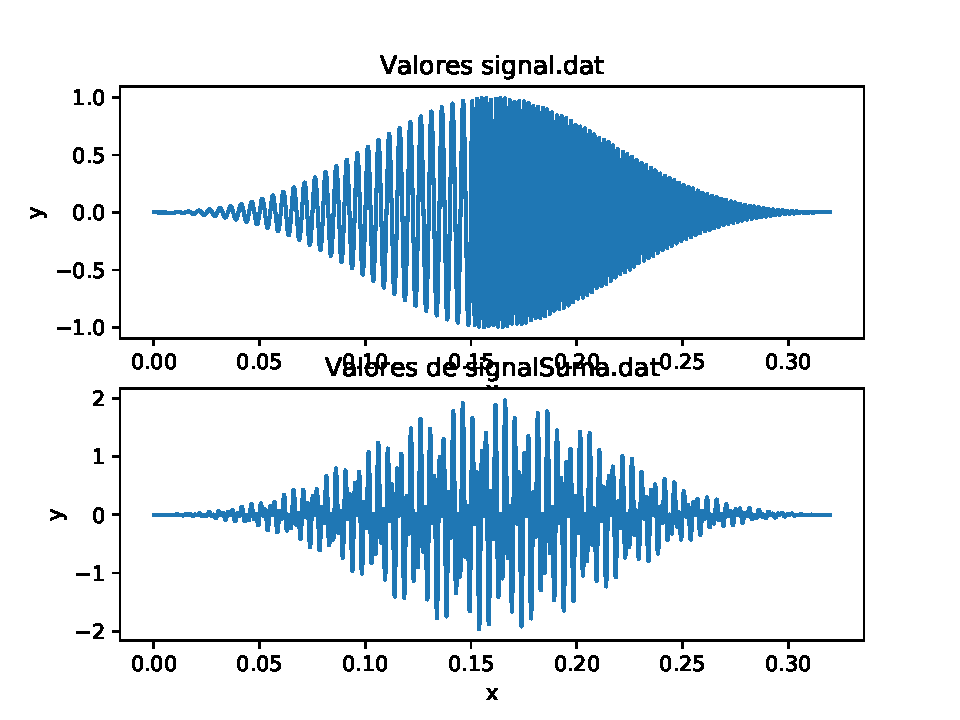
\includegraphics[width=13cm, height=7cm]{GarciaCamila_SubplotsGraficas.pdf}\\
\small{Figura 1: Grafica con los datos de signal.dat y signalSuma.dat.}
\end{center}

A continuacion se tienen la grafica de de las transformadas de fourier para ambas señales. 

\begin{center}
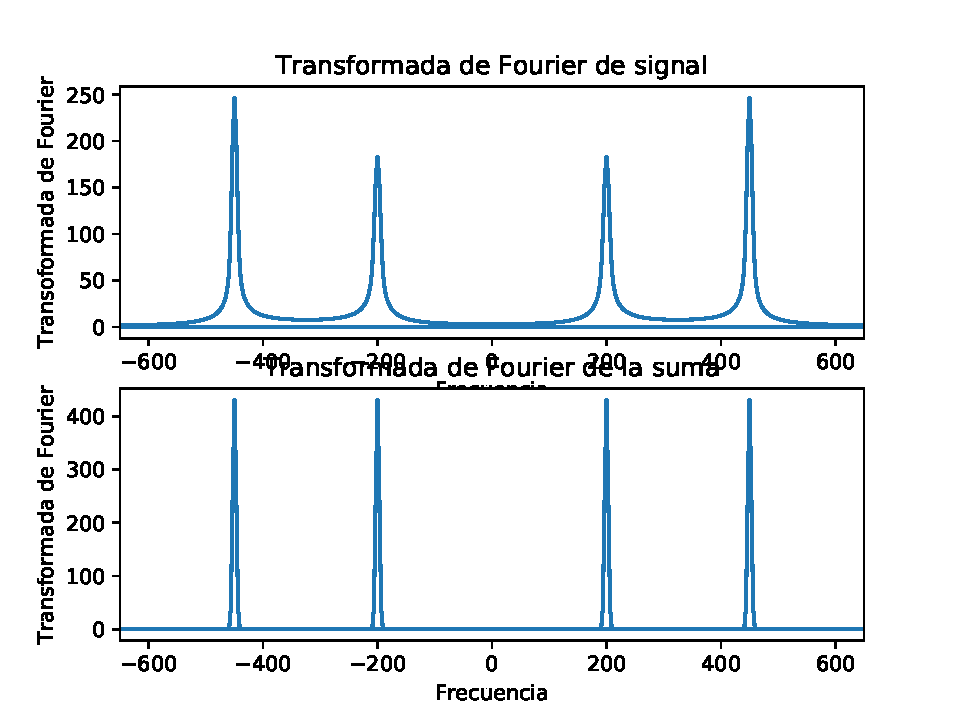
\includegraphics[width=13cm, height=7cm]{GarciaCamila_Transformadas.pdf}\\
\small{Figura 2: Grafica con las transformadas de fourier de los datos de signal.dat y signalSuma.dat.}
\end{center}

Posteriormente, se muestra el espectograma de los datos.

\begin{center}
\includegraphics[width=13cm, height=7cm]{GarciaCamila_Espectogramas.pdf}\\
\small{Figura 3: Espectogramas de los datos de signal.dat y signalSuma.dat.}
\end{center}

Ahora se tiene la transformada de Fourier de los datos temblor.txt.

\begin{center}
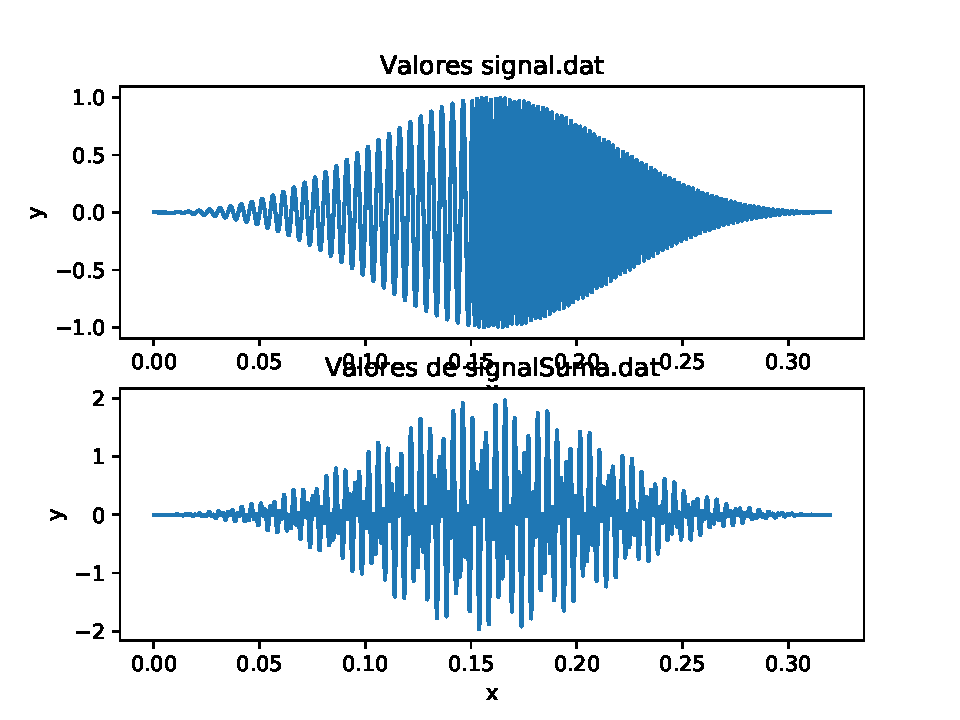
\includegraphics[width=13cm, height=7cm]{GarciaCamila_SubplotsGraficas.pdf}\\
\small{Figura 4: Grafica con los datos de signal.dat y signalSuma.dat.}
\end{center}

Finalmente, se tiene el espectograma de la señal temblor.txt.

\begin{center}
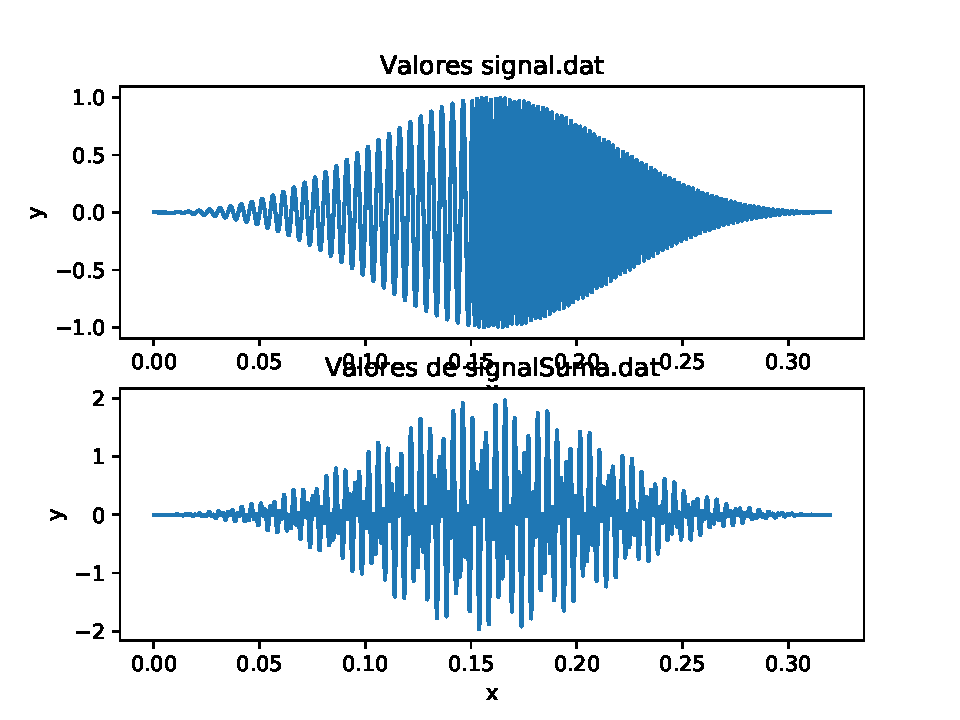
\includegraphics[width=13cm, height=7cm]{GarciaCamila_SubplotsGraficas.pdf}\\
\small{Figura 5: Espectograma de la señal temblor.txt.}
\end{center}
